\section{Results}
\label{sec:results}

\subsection{Transfer Performance}
\Tabref{tab:transfer} summarizes zero-shot transfer.
Mean drops range from 7.2 points (\sib, \xlmr) to 19.9 points (NER, \mbert), with large spread across languages; this spread is what the predictors must explain.
The seed standard deviation of a language's score averages 0.4 points (\xnli) to 1.7 points (NER), small relative to the between-language spread.
On whitespace-segmented targets, fertility ratios range from 0.92 to 3.80 for \mbert (median 1.64) and from 0.84 to 2.02 for \xlmr (median 1.31).
\xlmr's larger vocabulary fragments every language less than \mbert's.

\begin{table}[t]
    \centering
    \resizebox{0.9\textwidth}{!}{%
    \begin{tabular}{@{}llcrrrrl@{}}
        \toprule
        Task & Model & Seeds & English & Mean target & Mean drop & SD of drop & Largest drop \\
        \midrule
        \xnli    & \mbert & 3 & 78.1 & 64.3 & 13.8 & 6.7  & 27.4 (\lang{sw}) \\
                 & \xlmr  & 3 & 80.9 & 70.8 & 10.0 & 4.0  & 17.2 (\lang{sw}) \\
        \midrule
        \wikiann NER & \mbert & 3 & 84.4 & 64.6 & 19.9 & 15.2 & 83.8 (\lang{th}) \\
                 & \xlmr  & 3 & 82.8 & 64.6 & 18.2 & 15.5 & 79.0 (\lang{th}) \\
        \midrule
        \sib     & \mbert & 5 & 88.5 & 76.5 & 12.1 & 9.0  & 36.5 (\lang{mg}) \\
                 & \xlmr  & 5 & 89.5 & 82.4 & 7.2  & 5.5  & 27.0 (\lang{ga}) \\
        \bottomrule
    \end{tabular}
    }
    \caption{
        Zero-shot transfer performance over all target languages (14 for \xnli, 71 for NER and \sib).
        Scores are accuracy (\xnli, \sib) or span F1 (NER), averaged over seeds; drops are in points relative to English.
        Uniform chance is 33\% for \xnli and 14\% for \sib.
    }
    \label{tab:transfer}
\end{table}


\subsection{H1 and H2: Variance Explained}

\begin{figure}[t]
    \centering
    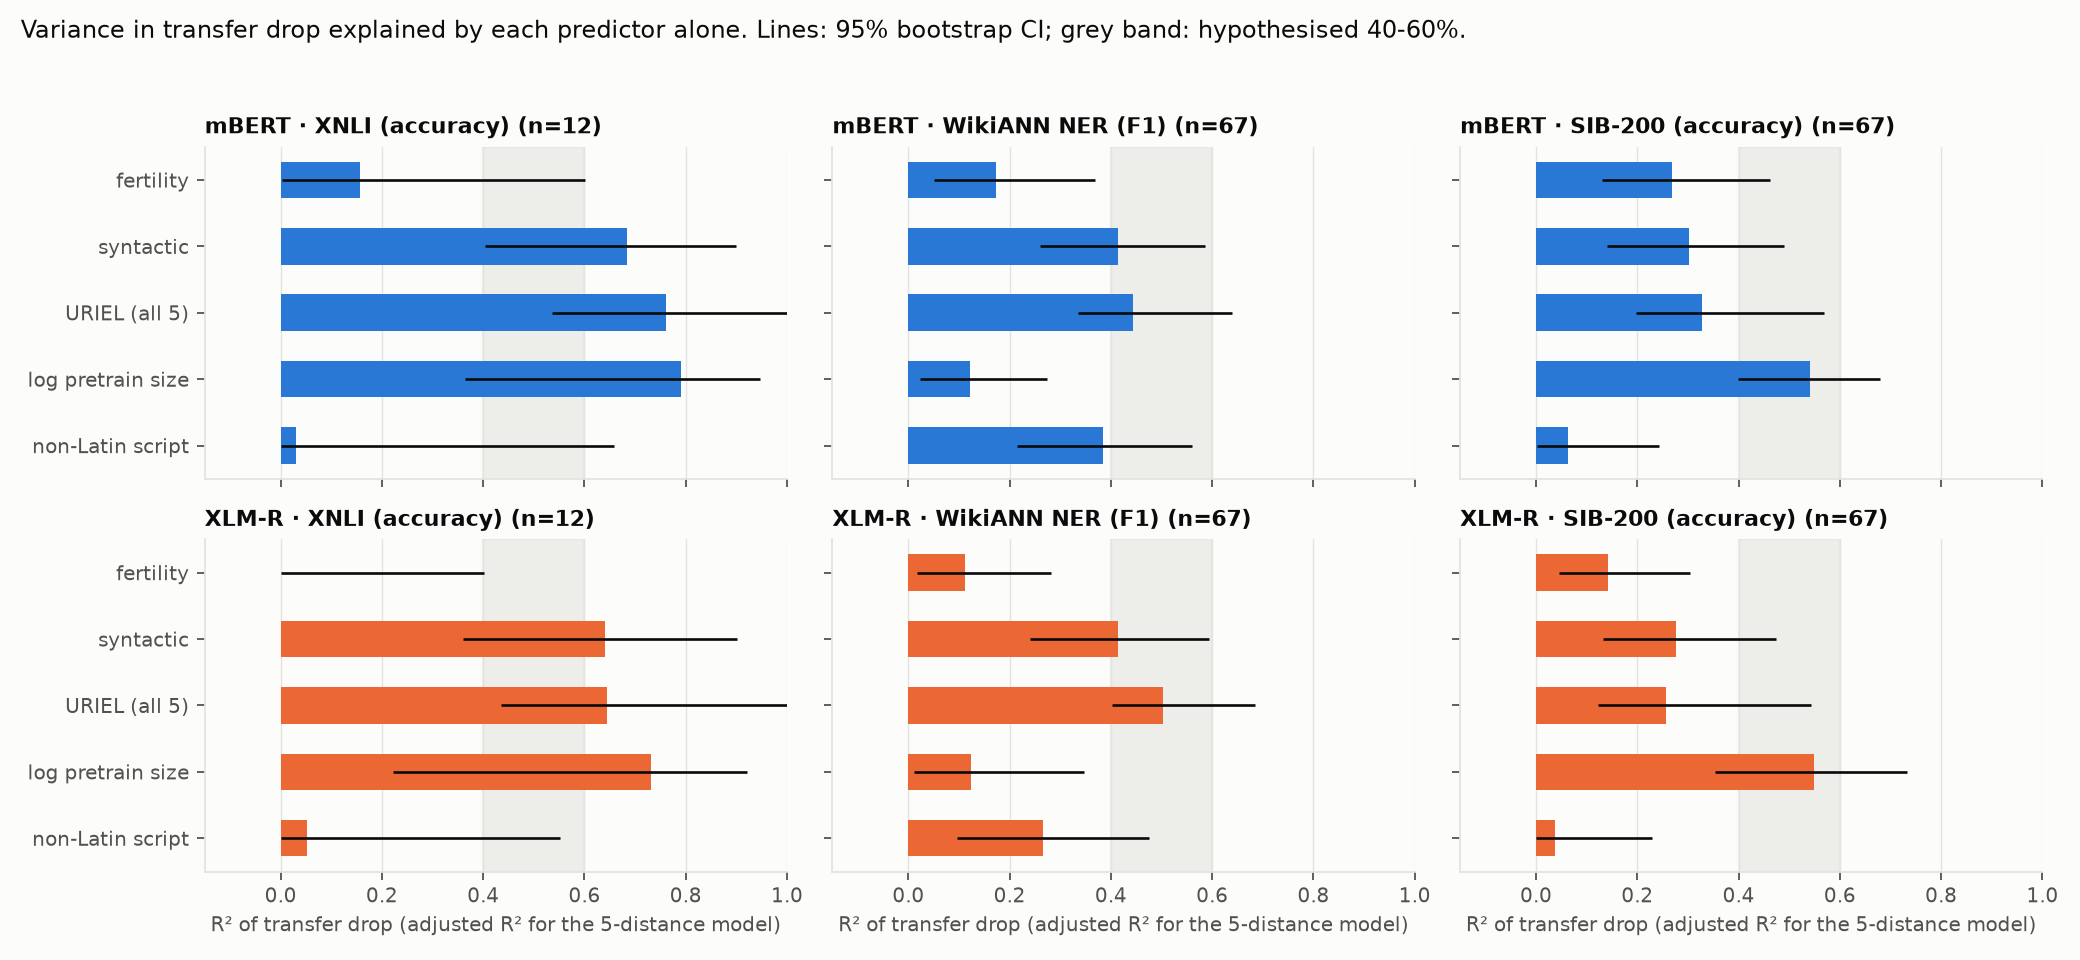
\includegraphics[width=0.95\linewidth]{figures/fig2_r2_by_predictor.png}
    \caption{
        \rsq of transfer drop for each predictor alone, by model (rows) and task (columns).
        Lines show 95\% bootstrap confidence intervals and the grey band marks the hypothesized 40--60\% range.
        The fertility bar falls short of the band in every panel, while syntactic distance or log pretraining size reaches or exceeds it in most.
    }
    \label{fig:r2}
\end{figure}

\begin{table}[t]
    \centering
    \resizebox{\textwidth}{!}{%
    \begin{tabular}{@{}llrlllcl@{}}
        \toprule
             &       &     & \multicolumn{2}{c}{Single predictor} & & Joint model & \\
        \cmidrule(lr){4-5} \cmidrule(lr){7-7}
        Task & Model & $n$ & Fertility & Syntactic distance & log pretrain size & \uriel, all 5 (adj.) & Non-Latin script \\
        \midrule
        \xnli & \mbert & 12 & 0.16 [0.00, 0.60] & 0.68 [0.40, 0.90] & {\bf 0.79} [0.36, 0.95] & 0.76 & 0.03 \\
              & \xlmr  & 12 & 0.00 [0.00, 0.40] & 0.64 [0.36, 0.90] & {\bf 0.73} [0.22, 0.92] & 0.65 & 0.05 \\
        \midrule
        NER   & \mbert & 67 & 0.17 [0.05, 0.37] & {\bf 0.41} [0.26, 0.59] & 0.12 [0.02, 0.27] & 0.44 & 0.38 \\
              & \xlmr  & 67 & 0.11 [0.02, 0.28] & {\bf 0.41} [0.24, 0.59] & 0.12 [0.01, 0.35] & 0.50 & 0.27 \\
        \midrule
        \sib  & \mbert & 67 & 0.27 [0.13, 0.46] & 0.30 [0.14, 0.49] & {\bf 0.54} [0.40, 0.68] & 0.33 & 0.06 \\
              & \xlmr  & 67 & 0.14 [0.05, 0.30] & 0.28 [0.13, 0.47] & {\bf 0.55} [0.35, 0.73] & 0.26 & 0.04 \\
        \midrule
        \multicolumn{2}{@{}l}{Pooled (292 rows)} & 67 & 0.16 [0.07, 0.28] & {\bf 0.37} [0.26, 0.48] & 0.32 [0.19, 0.46] & -- & -- \\
        \bottomrule
    \end{tabular}
    }
    \caption{
        \rsq of transfer drop for each predictor alone, with 95\% bootstrap confidence intervals in brackets.
        Fertility never reaches the hypothesized 40--60\% and is below syntactic distance in all six cells.
        The best of the three main single predictors is in \textbf{bold}.
        The joint \uriel column reports adjusted \rsq for a model with five distances.
        The pooled row z-scores drops within cell and clusters the bootstrap by language.
    }
    \label{tab:r2}
\end{table}


\para{H1 is not supported.}
\Tabref{tab:r2} and \figref{fig:r2} show that no fertility point estimate falls in the 40--60\% range; the values are 0.00--0.27.
The upper confidence bound reaches 0.40 only where the interval is widest: the two 12-language \xnli cells (0.60 and 0.40) and \sib with \mbert (0.46).
The association is nonetheless real in the larger cells.
On NER and \sib, Pearson $r$ is 0.33--0.52 and Spearman $\rho$ is 0.40--0.66, all with Holm-adjusted $p<0.02$.
On \xnli it is not distinguishable from zero ($r=0.40$ and $-0.03$, $n=12$).
\Figref{fig:scatter} shows the underlying scatter.

\para{H2 is not supported; the sign is reversed.}
Fertility \rsq is below syntactic-distance \rsq in all six cells.
The bootstrap interval of the difference excludes zero in four cells (both \xnli and both NER cells, with differences of $-0.24$ to $-0.64$); after Holm correction only NER with \xlmr stays below 0.05.
On \sib the two predictors are statistically indistinguishable (differences of $-0.03$ and $-0.13$).
Which baseline is strongest depends on the task: log pretraining size is the best single predictor on \xnli and \sib, and syntactic distance on NER, where size and fertility are tied at low values.

\para{Pooled estimate.}
Over 292 language--cell rows from 67 languages, fertility explains 0.16 [0.07, 0.28], syntactic distance 0.37 [0.26, 0.48] and log size 0.32 [0.19, 0.46].
The difference between fertility and syntactic distance is $-0.21$ [$-0.33$, $-0.08$].

\begin{figure}[t]
    \centering
    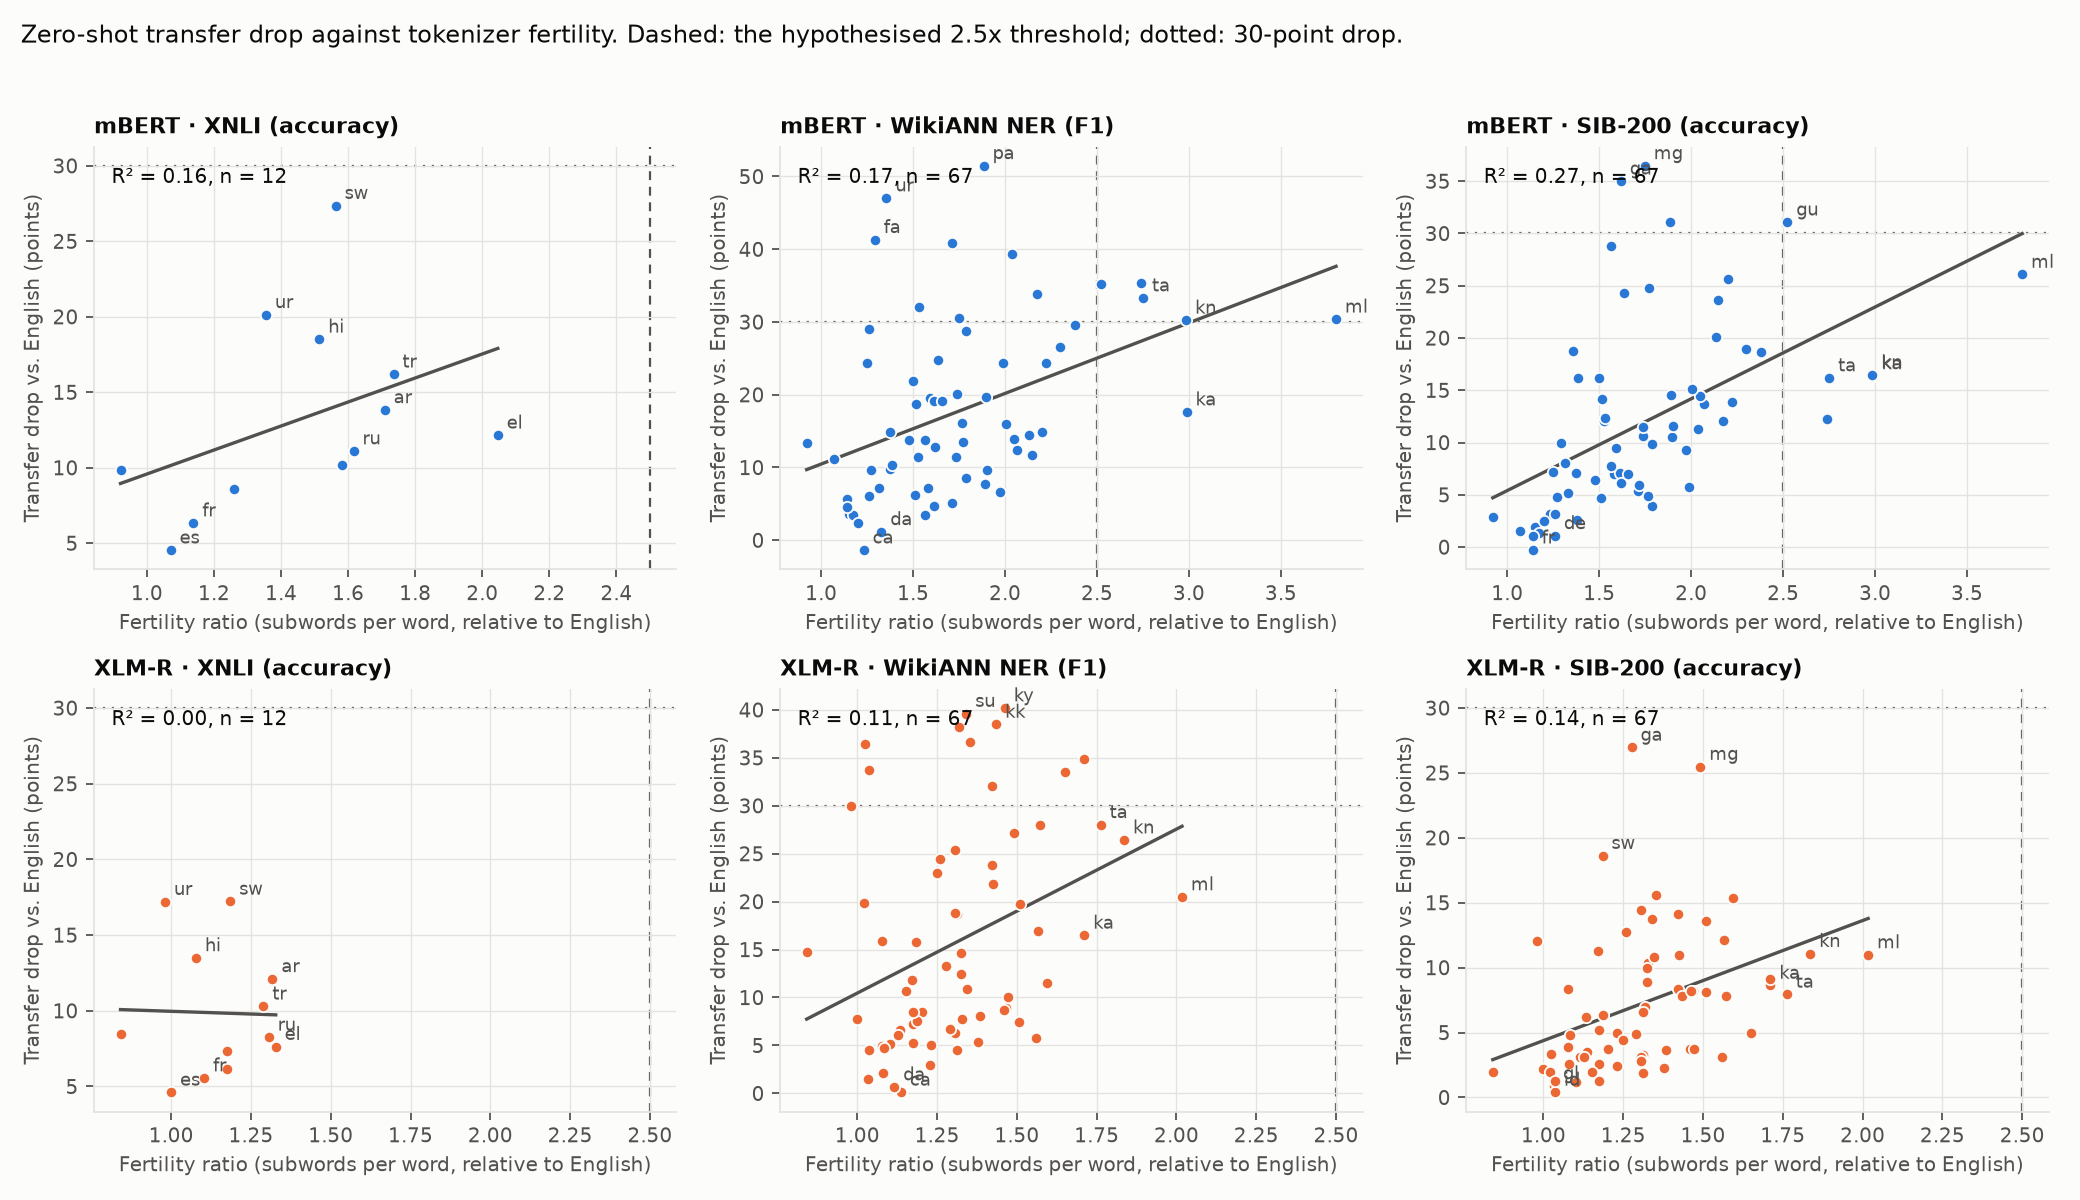
\includegraphics[width=0.95\linewidth]{figures/fig1_fertility_vs_drop.png}
    \caption{
        Transfer drop against fertility ratio for each language, with the OLS fit.
        The dashed line marks the hypothesized 2.5$\times$ threshold and the dotted line a 30-point drop.
        Many languages with low fertility have large drops (\eg \lang{ur}, \lang{fa}, \lang{sw}, \lang{mg}), and no language exceeds 2.5$\times$ under \xlmr (bottom row).
    }
    \label{fig:scatter}
\end{figure}

\subsection{H3: The 2.5$\times$ Threshold}

\begin{table}[t]
    \centering
    \resizebox{\textwidth}{!}{%
    \begin{tabular}{@{}lllllc@{}}
        \toprule
        Cell & Languages above 2.5$\times$ & Above: drop $>30$ & Below: drop $>30$ & Mean drop above / below & Fisher $p$ \\
        \midrule
        NER, \mbert   & 6 (\lang{gu ka kn ml ta te}) & 5 of 6 & 8 of 61 & 30.4 / 16.5 & 0.001 \\
        \sib, \mbert  & same 6 & 1 of 6 & 3 of 61 & 19.7 / 11.2 & 0.32 \\
        \xnli, \mbert & 0 of 12 & -- & 0 of 12 & -- & -- \\
        NER, \xlmr    & 0 of 67 & -- & 10 of 67 & -- & -- \\
        \sib, \xlmr   & 0 of 67 & -- & 0 of 67 & -- & -- \\
        \xnli, \xlmr  & 0 of 12 & -- & 0 of 12 & -- & -- \\
        \bottomrule
    \end{tabular}
    }
    \caption{
        The 2.5$\times$ threshold on whitespace-segmented targets.
        Only \mbert's tokenizer produces any language above the threshold, and those six languages fail on NER but not on topic classification.
    }
    \label{tab:threshold}
\end{table}


\Tabref{tab:threshold} tests the threshold claim.
Under \xlmr's tokenizer no whitespace-segmented language exceeds 2.02$\times$, so we cannot test the claim there; yet 10 languages still lose more than 30 F1 on NER.
Under \mbert, six languages exceed 2.5$\times$.
NER fits the claim (5 of 6 fail above the threshold against 8 of 61 below; Fisher $p=0.001$), but topic classification does not (1 of 6 against 3 of 61; $p=0.32$), and the mean \sib drop above the threshold is 19.7 points.

We find no break at 2.5.
Adding a hinge at 2.5 to the linear fit does not help, and its coefficient is negative (NER $p=0.33$, \sib $p=0.07$); if anything, the slope flattens.

The NER result is also entangled with script.
All six languages above 2.5$\times$ use Brahmic or Georgian scripts.
In a post hoc check, 6 of the 21 non-Latin targets with fertility \emph{below} 2.5 also lose more than 30 F1, including the four largest drops in the cell (\lang{pa}, \lang{ur}, \lang{fa}, \lang{ar}, at fertility 1.3--1.9), against 2 of 40 Latin-script targets.
With the parallel token ratio over all 71 targets, three languages exceed 2.5 for \mbert (\lang{ml}, \lang{my}, \lang{th}); all three fail on NER and none on \sib.
We conclude that H3 is not supported as a general rule; the data are consistent with it in one cell of six.

\subsection{H4: Independence from Pretraining Size}

\begin{table}[t]
    \centering
    \resizebox{\textwidth}{!}{%
    \begin{tabular}{@{}llrrrrc@{}}
        \toprule
             &       &                       & \multicolumn{3}{c}{Partial $r$ of fertility with drop, given} & Unique \rsq \\
        \cmidrule(lr){4-6}
        Task & Model & $r$(fert., size) & size & size + syntactic & size + syntactic + script & fert.\ / size / syntactic \\
        \midrule
        \xnli & \mbert & $-0.29$ & 0.32 (0.68)        & 0.38 (1.0)         & 0.26 (1.0)    & 0.02 / 0.12 / 0.05 \\
              & \xlmr  & 0.00    & $-0.05$ (0.89)     & $-0.03$ (1.0)      & $-0.24$ (1.0) & 0.00 / 0.16 / 0.07 \\
        \midrule
        NER   & \mbert & $-0.33$ & {\bf 0.34} (0.026) & 0.09 (1.0)         & $-0.22$ (0.38) & 0.005 / 0.001 / 0.20 \\
              & \xlmr  & $-0.33$ & 0.25 (0.18)        & 0.02 (1.0)         & $-0.11$ (1.0)  & 0.00 / 0.005 / 0.24 \\
        \midrule
        \sib  & \mbert & $-0.33$ & {\bf 0.43} (0.002) & {\bf 0.34} (0.031) & 0.28 (0.16)    & 0.05 / 0.27 / 0.01 \\
              & \xlmr  & $-0.33$ & 0.21 (0.27)        & 0.09 (1.0)         & 0.08 (1.0)     & 0.004 / 0.31 / 0.03 \\
        \bottomrule
    \end{tabular}
    }
    \caption{
        Does fertility carry information beyond pretraining size?
        Holm-adjusted $p$-values in parentheses; partial correlations with adjusted $p<0.05$ in \textbf{bold}.
        Unique \rsq is the loss in \rsq when a predictor is removed from the model with fertility, log size and syntactic distance.
        Fertility's unique contribution never exceeds 0.05.
    }
    \label{tab:partial}
\end{table}


\Tabref{tab:partial} shows that fertility and pretraining size are only moderately correlated ($r\approx-0.3$), so the fertility association is not simply a size effect.
Given size alone, the partial correlation stays positive in five cells and is significant in two.
Given size \emph{and} syntactic distance, it is significant in one cell (\sib with \mbert), and fertility's unique contribution is at most 0.05 of \rsq everywhere.
We find no fertility $\times$ size interaction in any cell (all $p>0.1$).
H4 is therefore supported only in a narrow sense: size alone does not explain the association away, but fertility carries little information beyond size and syntax together.

\subsection{Within-Language Contrast}

\begin{figure}[t]
    \centering
    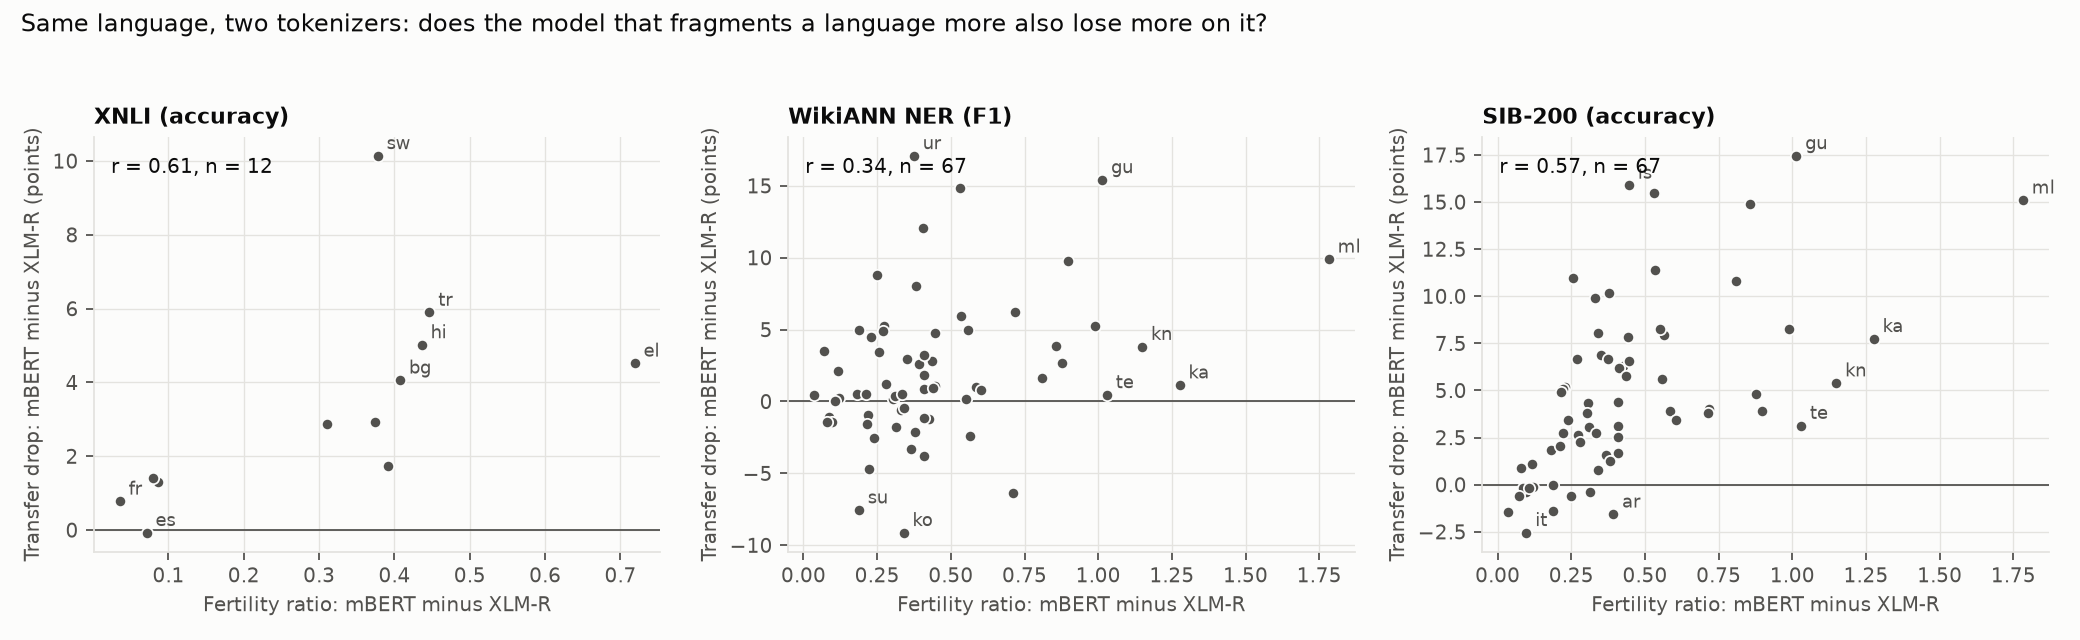
\includegraphics[width=0.95\linewidth]{figures/fig3_within_language_contrast.png}
    \caption{
        Within-language contrast.
        Each point is one language; the x-axis is how much more \mbert fragments it than \xlmr, and the y-axis is how much more \mbert loses on it.
        The relationship is positive on all three tasks ($r=0.61$, 0.34, 0.57).
    }
    \label{fig:within}
\end{figure}

\begin{table}[t]
    \centering
    \begin{tabular}{@{}lrlcl@{}}
        \toprule
        Task & $n$ & Pearson $r$ [95\% CI] & Spearman $\rho$ & Partial $r$ given size difference \\
        \midrule
        \xnli & 12 & 0.61 [0.30, 0.93] & 0.83 & 0.59 ($p=0.056$) \\
        NER   & 67 & 0.34 [0.13, 0.53] & 0.36 & 0.34 ($p=0.006$) \\
        \sib  & 67 & 0.57 [0.38, 0.71] & 0.64 & 0.57 ($p<0.001$) \\
        \bottomrule
    \end{tabular}
    \caption{
        Within-language contrast: correlation between the fertility difference (\mbert minus \xlmr) and the drop difference (\mbert minus \xlmr) across languages.
        The language, its typology and its test data are the same on both sides of each difference.
    }
    \label{tab:within}
\end{table}


For a given language, the more \mbert fragments it relative to \xlmr, the larger \mbert's extra drop (\figref{fig:within}, \tabref{tab:within}).
The correlation is 0.61 on \xnli, 0.34 on NER and 0.57 on \sib, and it barely changes when we control for the difference in pretraining size.
Typology is fixed by construction, so this is the strongest observational evidence here for a fertility effect.
It does not isolate segmentation, however: the two models also differ in pretraining corpus, objective and training budget.

\subsection{Intervention: Over-Segmenting English}

\begin{figure}[t]
    \centering
    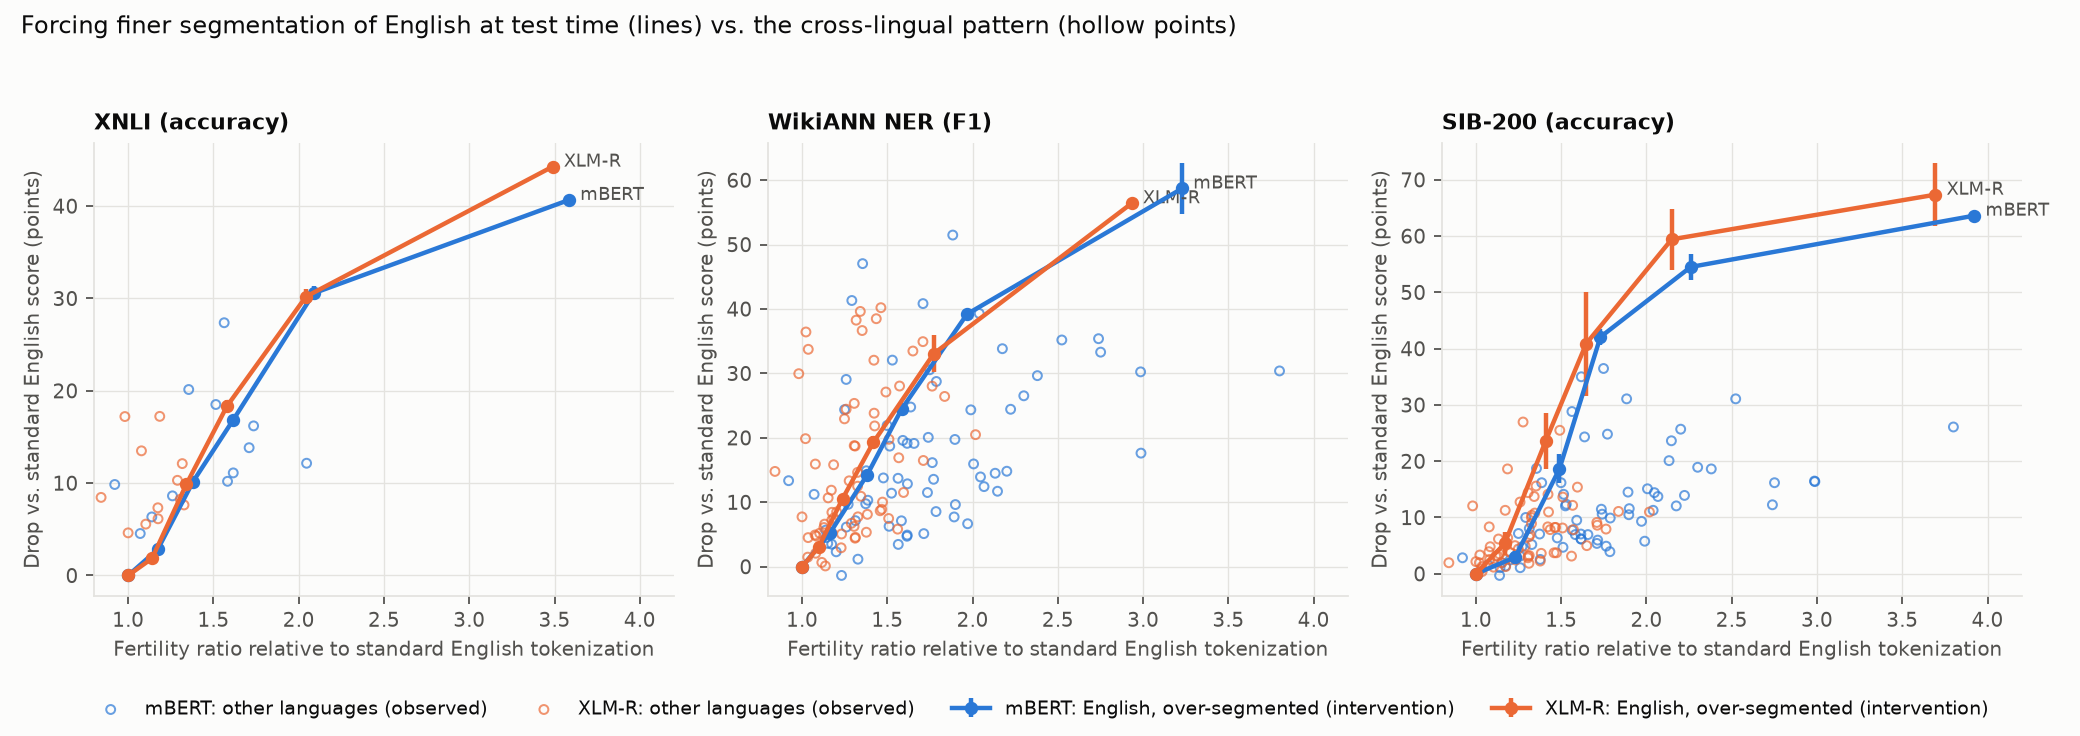
\includegraphics[width=0.95\linewidth]{figures/fig4_intervention.png}
    \caption{
        Drop in English score when we force finer segmentation at test time (lines, with seed SD), compared with the observed drops of other languages at their natural fertility (hollow points).
        The loss grows monotonically and steeply, and on \sib over-segmented English does far worse than natural languages at the same fertility.
    }
    \label{fig:intervention}
\end{figure}

\begin{table}[t]
    \centering
    \resizebox{0.9\textwidth}{!}{%
    \begin{tabular}{@{}lccccccc@{}}
        \toprule
                           &                 & \multicolumn{2}{c}{\xnli} & \multicolumn{2}{c}{NER} & \multicolumn{2}{c}{\sib} \\
        \cmidrule(lr){3-4} \cmidrule(lr){5-6} \cmidrule(lr){7-8}
        Max subword length & Fertility ratio & \mbert & \xlmr & \mbert & \xlmr & \mbert & \xlmr \\
        \midrule
        6 chars & 1.1--1.2 & 2.8  & 1.8  & 5.2  & 3.0  & 2.9  & 5.4 \\
        4 chars & 1.2--1.5 & 10.2 & 9.9  & 14.3 & 10.6 & 18.6 & 23.6 \\
        3 chars & 1.4--1.7 & 16.8 & 18.3 & 24.4 & 19.3 & 42.1 & 40.9 \\
        2 chars & 1.8--2.3 & 30.6 & 30.2 & 39.2 & 33.1 & 54.5 & 59.4 \\
        1 char  & 2.9--3.9 & 40.7 & 44.3 & 58.7 & 56.4 & 63.6 & 67.4 \\
        \bottomrule
    \end{tabular}
    }
    \caption{
        Drop in English test score (points) when we cap the length of every subword at test time.
        The fertility ratio is relative to standard English tokenization and varies by model and task.
        Values are means over seeds; seed SD is under 1 point for \xnli, up to 4 for NER and up to 9 for \sib.
        At the 1-character cap, 8\% (\sib) and 18--19\% (\xnli) of tokens are also truncated by the length limit.
    }
    \label{tab:intervention}
\end{table}


Finer segmentation of the same English text causes a monotonic, steep loss in every cell (\tabref{tab:intervention}, \figref{fig:intervention}).
A 4-character cap, which raises fertility to 1.2--1.5$\times$, costs 10--24 points; a 2-character cap, at 1.8--2.3$\times$, costs 30--59 points.
At equal fertility the loss can be much larger than the cross-lingual regression line predicts.
On \sib with \mbert at 1.73$\times$, over-segmented English loses 42 points, against about 12 for a typical language at that fertility.
Real high-fertility languages do much better than over-segmented English.

{\bf What does the intervention measure?}
It shows that segmentation granularity has a causal effect on these models, with a caveat about what kind.
The forced pieces are sequences the model rarely or never saw for those words in pretraining or fine-tuning, so the intervention measures the cost of \emph{unfamiliar} fragmentation.
A language that is naturally fragmented was pretrained in that form.
The gap between the intervention curve and the cross-lingual points suggests that pretraining exposure absorbs most of the cost, which fits fertility being a weak cross-lingual predictor.
This reading is an interpretation; no experiment here tests it directly.
At the 1-character cap the two sentence-level tasks also mix fragmentation with truncation; at 2 characters and above, truncation is under 1\%.

\subsection{Robustness and Exploratory Results}

\begin{table}[t]
    \centering
    \resizebox{\textwidth}{!}{%
    \begin{tabular}{@{}lcccccc@{}}
        \toprule
                & \multicolumn{2}{c}{\xnli} & \multicolumn{2}{c}{NER} & \multicolumn{2}{c}{\sib} \\
        \cmidrule(lr){2-3} \cmidrule(lr){4-5} \cmidrule(lr){6-7}
        Variant & \mbert & \xlmr & \mbert & \xlmr & \mbert & \xlmr \\
        \midrule
        Primary (subwords per word, linear)                  & 0.16 & 0.00 & 0.17 & 0.11 & 0.27 & 0.14 \\
        log fertility                                        & 0.19 & 0.00 & 0.18 & 0.10 & 0.31 & 0.15 \\
        Parallel token ratio, all targets                    & 0.33 & 0.01 & 0.27 & 0.00 & {\bf 0.51} & {\bf 0.42} \\
        Parallel token ratio, segmented targets (post hoc)   & 0.14 & 0.00 & 0.22 & 0.03 & {\bf 0.50} & {\bf 0.44} \\
        Fertility measured on \wikiann words                 & --   & --   & 0.36 & 0.28 & --   & --   \\
        NER test sets of 1{,}000+ sentences                  & --   & --   & 0.16 & 0.09 & --   & --   \\
        Latin-script targets only                            & 0.52$^\dagger$ & 0.15$^\dagger$ & 0.04 & 0.03 & 0.32 & 0.18 \\
        Non-Latin targets only                               & 0.34$^\dagger$ & 0.49$^\dagger$ & 0.00 & 0.01 & 0.23 & 0.07 \\
        \bottomrule
    \end{tabular}
    }
    \caption{
        \rsq of transfer drop on fertility under alternative definitions and subsets.
        Values inside the hypothesized 40--60\% range with $n=67$ or more are in \textbf{bold}.
        $^\dagger$~$n=6$ languages.
    }
    \label{tab:robustness}
\end{table}


\Tabref{tab:robustness} reports \rsq under alternative definitions and subsets.
The primary conclusion does not depend on linear versus log fertility, or on the ten NER test sets with only 100 sentences.

\para{The fertility definition matters on \sib.}
The parallel token ratio explains 42--51\% of the variance there, inside the hypothesized range.
It keeps a partial correlation of 0.45--0.60 after controlling for size, syntactic distance and script (uncorrected $p<0.001$).
This is not due to the four added unsegmented languages, since it holds on the same 67 targets.
On NER and \xnli the same measure does no better than the primary one, and pretraining size still matches or exceeds it on \sib (0.55--0.56).
The \sib test sentences are themselves \flores sentences, so here the parallel ratio is measured on the same text distribution as the task, which may be part of why it works.
The measure was pre-specified as secondary, but its decomposition is post hoc and it is one of several variants, so we treat it as a lead and not as a confirmation.

\para{In-domain fertility is a better measurement.}
Measuring fertility on \wikiann's own words roughly doubles \rsq on NER (0.36 and 0.28), still below syntactic distance (0.41).

\para{On NER, fertility is a between-script difference.}
Within either script group, fertility explains essentially nothing on NER (0.00--0.04), so its cell-level \rsq of 0.11--0.17 reflects the difference between Latin and non-Latin targets.

\para{Measurement noise.}
With 204 test sentences per language, binomial sampling accounts for 17\% (\mbert) and 38\% (\xlmr) of the between-language variance in \sib drops, which caps any predictor's \rsq near 0.83 and 0.62.
Pretraining size (0.54, 0.55) is close to that ceiling for \xlmr; fertility (0.27, 0.14) is not.
\xnli drops are 96--98\% reliable.

\subsection{Error Analysis: Where Fertility Mispredicts}
We inspect the residuals of the fertility regression and find three patterns.

\para{Low fertility, large drop.}
Urdu, Persian, Arabic, Swahili, Malagasy and Irish lose far more than fertility predicts: on NER with \mbert, the residuals are $+33$ for Urdu, $+32$ for Punjabi, $+28$ for Persian and $+23$ for Arabic, and on \sib $+24$ for both Malagasy and Irish.
These languages are tokenized compactly but are syntactically distant, low-resource, or (for NER) written in Arabic script.
\xlmr tokenizes Urdu at 0.98$\times$ English and still loses 17 points on \xnli.

\para{High fertility, small drop.}
Finnish, Hungarian, Korean and Telugu lose less than fertility predicts.
These agglutinative, well-resourced languages are fragmented heavily and transfer fine.

\para{Task dependence.}
NER residuals split by script (mean about $+5$ for non-Latin and $-4$ for Latin targets), whereas sentence-classification residuals do not (within 1 point).
